% wham_controllers_sop.tex -- unified Standard Operating Procedure for the WHAM controllers (XREX and HBRIDGE).
%
% STATUS: SKELETON (2026-11-18). The structure is final; the content is bullets of known facts, each with its
% source, for the owner to expand into prose. \todo{...} marks what only the owner can supply; every \todo is
% listed in the appendix "Owner input needed". Build: pdflatex wham_controllers_sop.tex (twice), then look at
% the pages (pdftoppm -r 60 -png ...). House style follows the former per-product SOPs (mathpazo, 5in x 8.25in,
% \tabcolsep 4pt to keep wide tables inside the margin).
\documentclass[11pt]{article}

\usepackage{color,hyperref,amsmath}
\usepackage[sc,osf]{mathpazo}
\usepackage[a4paper, total={6in, 8.25in}]{geometry}
\usepackage[utf8]{inputenc}
\usepackage{graphicx}
\usepackage{float}
\usepackage{longtable}
\usepackage{array}
\newcolumntype{L}[1]{>{\raggedright\arraybackslash}p{#1}}
\usepackage{enumitem}
\usepackage{tikz}
\usetikzlibrary{positioning}
\usepackage{varwidth}

\hypersetup{colorlinks=true, linkcolor=blue, urlcolor=blue}
\setlength{\emergencystretch}{2em}
\setlength{\tabcolsep}{4pt}
\setlist{nosep, leftmargin=1.4em}

\newcommand{\code}[1]{\texttt{#1}}
\newcommand{\file}[1]{\nolinkurl{#1}}
\newcommand{\src}[1]{{\scriptsize\textcolor[gray]{0.45}{[src: #1]}}}
\newcommand{\cl}[2]{\texttt{#1}\hfill$\to$~\texttt{#2}}

\newcommand{\caution}[1]{\par\noindent\fbox{\parbox{4.85in}{\textbf{CAUTION:} #1}}\par\smallskip}
\newcommand{\note}[1]{\par\noindent\fbox{\parbox{4.85in}{\textbf{NOTE:} #1}}\par\smallskip}

% \todo{text}: a visible, numbered placeholder for owner input, collected in the appendix list.
\makeatletter
\newcounter{todoc}
\newcommand{\todo}[1]{\refstepcounter{todoc}{\color{red}\fbox{\scriptsize OWNER~\thetodoc}}~\textit{#1}%
  \addcontentsline{tdo}{todoc}{\protect\numberline{\thetodoc}#1}}
\newcommand{\l@todoc}{\@dottedtocline{1}{0em}{2.3em}}
\newcommand{\listoftodos}{\@starttoc{tdo}}
\makeatother

% Procedure template: \begin{procedure} ... \end{procedure} with \pitem{Heading} entries.
\newenvironment{procedure}{\begin{description}[style=nextline, leftmargin=1.2em, font=\normalfont\bfseries]}{\end{description}}
\newcommand{\pitem}[1]{\item[#1]}

\title{WHAM Controllers (XREX and HBRIDGE)\\ \large Standard Operating Procedure\\ \normalsize Build, deployment, operation and maintenance}
\author{}
\date{Draft skeleton, 2026-11-18}

\begin{document}
\sloppy
\maketitle

\begin{center}
\begin{tabular}{L{0.35in} L{0.75in} L{0.5in} L{2.85in}}
  \hline
  \textbf{Rev} & \textbf{Date} & \textbf{Author} & \textbf{Description} \\
  \hline
  -- & 2026-11-18 & -- & Skeleton: structure and known facts as bullets; prose to be written. Supersedes (once complete)
    the per-product SOPs \file{firmware/xrex/docs/sop/} (last Rev~G, 2026-09-29) and
    \file{firmware/hbridge/docs/sop/} (last Rev~D, 2026-09-29). \\
  A & & & First issue of the unified SOP. \todo{Date, author and approver for Rev A} \\
  \hline
\end{tabular}
\end{center}

\noindent\textbf{Approvals.} \todo{Approver names, roles and signature block}

\tableofcontents
\newpage

% ======================================================================
\section*{How to read this document}
\addcontentsline{toc}{section}{How to read this document}
\begin{itemize}
  \item Part~I (overview and safety), Part~III (procedures), Part~IV (support) and the appendices are for everyone who
    operates or maintains the controllers.
  \item Part~II is the engineering description (hardware, firmware, interfacing). Operators may skip it.
  \item This SOP holds stable content (purpose, design, procedures, safety rules). Fast-changing facts are referenced, not
    copied: full command lists (\file{firmware/<product>/docs/command_reference.md}), network addresses
    (\file{docs/bench_devices.md}), firmware versions (\code{*IDN?}, the changelogs), open items
    (\file{handoff/08_open_items.md}), verification status (the changelog status tags).
  \item Conventions: commands in \code{code font}; a command line shows the expected reply as
    \cl{STATE?}{OK IDLE}; CAUTION and NOTE boxes; \texttt{<...>} is a value you supply.
  \item \todo{Document number and storage location of the controlled copy}
\end{itemize}

% ======================================================================
\part{Overview and safety}

\section{Purpose, scope and audience}
\label{sec:purpose}
\begin{itemize}
  \item Purpose: how to build, deploy, operate and maintain the WHAM controller board and its two firmware products.
  \item Covers both products (XREX, HBRIDGE), every board in service, from building firmware to running and checking a shot.
  \item Does not cover: supply-side high-voltage work, facility lockout/tagout, facility interlocks. \todo{Name the facility documents that do}
  \item Audience: operators and technicians (Parts I, III, IV) and the maintaining engineer (all parts).
  \src{handoff/README.md; former SOPs, Purpose and Scope}
\end{itemize}

\section{Safety and responsibilities}
\label{sec:safety}
\caution{These controllers drive real high-voltage, high-current supplies. A shot makes power electronics switch.}
\begin{itemize}
  \item Roles and authority: who may \code{ARM} and fire, who may flash firmware, who may switch protections off.
    \todo{Role names and who holds each}
  \item Never start output (\code{ARM}, \code{FIRE}, \code{SHOT:STARt}, \code{SOURce:RUN}, an external trigger edge) without
    the system owner's OK for that board. \src{handoff/00 \S1}
  \item The ECH-HVPS controller (WB-0001-8) is installed in its supply: no shots without the owner's OK; queries and settings
    only while \cl{STATE?}{OK IDLE}. \src{owner instruction 2026-11-16}
  \item Identify every board by \code{*IDN?} (product and \code{SN=}) before sending anything else; an unrelated
    high-voltage controller shares the lab subnet and port. \src{handoff/05 \S5.1; docs/bench\_devices.md}
  \item Ask before every firmware flash; confirm each time that the board is safe (bench, or supply de-energized).
  \item Never feed pre-written answers into a confirmation prompt (a real shot was once fired this way, 2026-09-14).
  \item Do not test timing-dependent refusals over the network (round trip about 65\,ms).
  \item Switching off a protection (\code{GDS:ENAble ... 0}, \code{GDS:POLarity}, \code{DEBUG:FAULT:BYPASS 1},
    \code{EXTernal:ENAble 0}, \code{FAULT:CLEar}) is a deliberate, recorded act.
  \item Lab HV practice and lockout are referenced, not reproduced. \todo{References to the lab HV and lockout procedures}
\end{itemize}

\section{Background: why this project exists}
\label{sec:background}
\begin{itemize}
  \item \todo{The WHAM experiment and where these supplies fit (magnets, limiter, ECH gyrotron)}
  \item \todo{What the controllers replace (the previous control system) and why it was replaced}
  \item Hardware goals: one controller board for several supply types; fiber-optic isolation of drive, feedback and fault
    signals; remote operation over the lab network. \src{handoff/01 \S1.1}
  \item Firmware goals: precise multi-channel timing on the HRTIM; closed-loop control; safe remote firmware update; saved
    profiles; board identity; a strict, scriptable command protocol. \src{handoff/01 \S1.4}
  \item Two products on one board: XREX (four Transrex ISR-2126 magnet supplies, PFM, PID) and HBRIDGE (the HVPS, a three-phase
    H-bridge driven by PFM; the Limiter, single-phase PWM outputs, one per electrode: one electrode today, up to three, each with its own duty). \src{firmware/*/AGENTS.md, ``What this project is''}
  \item Keep this section to about one page.
\end{itemize}

There are three primary applications contributing to the design of the PFM-G474 controller:
\begin{center}
\begin{varwidth}{\textwidth}
\begin{enumerate}
	\item Limiter power supply: duty-cycle-controlled H-bridge;
	\item Gyrotron high-voltage power supply (HVPS): frequency-driven H-bridge;
	\item Transrex power supplies: frequency-driven (XREX), 4 instances.
\end{enumerate}
\end{varwidth}
\end{center}

An early version of the HVPS controller (\textit{Gyrotron HVPS Controller I/O Board V2, deprecated}) was developed in 2025 by Benjamin Terranova as part of the HVPS upgrade project led by Oscar Anderson. Ben designed the \textit{V2} controller around the STM32 Nucleo-L496ZG-P board, which could reliably produce 10--30\,kHz three-phase square waveforms with frequency sweeps, generating each signal and its complement. Due to the limitations of the L496ZG-P, this version of the controller could not eliminate so-called ``startup jitters'' at the beginning of a square-wave pulse (Figure~\ref{fig:v2-jitter}), which can produce phase imbalances early in the pulse and saturate the HVPS transformer cores.

\begin{figure}[H]
  \centering
  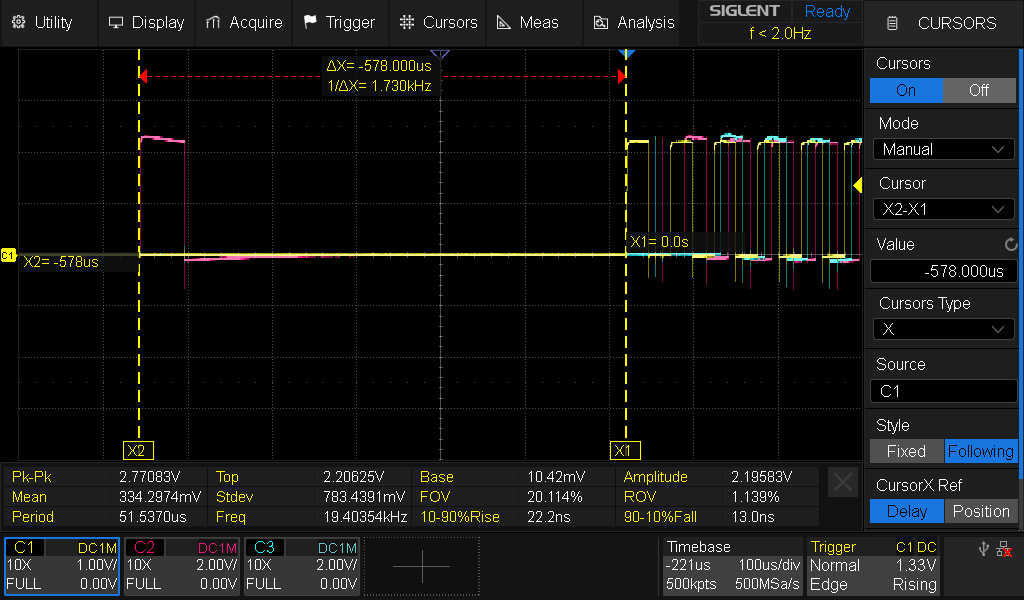
\includegraphics[width=0.75\linewidth]{img/V2_Startup_Jitters_01.png}\\[0.5ex]
  {\small (a) 100\,$\mu$s/div}\\[1ex]
  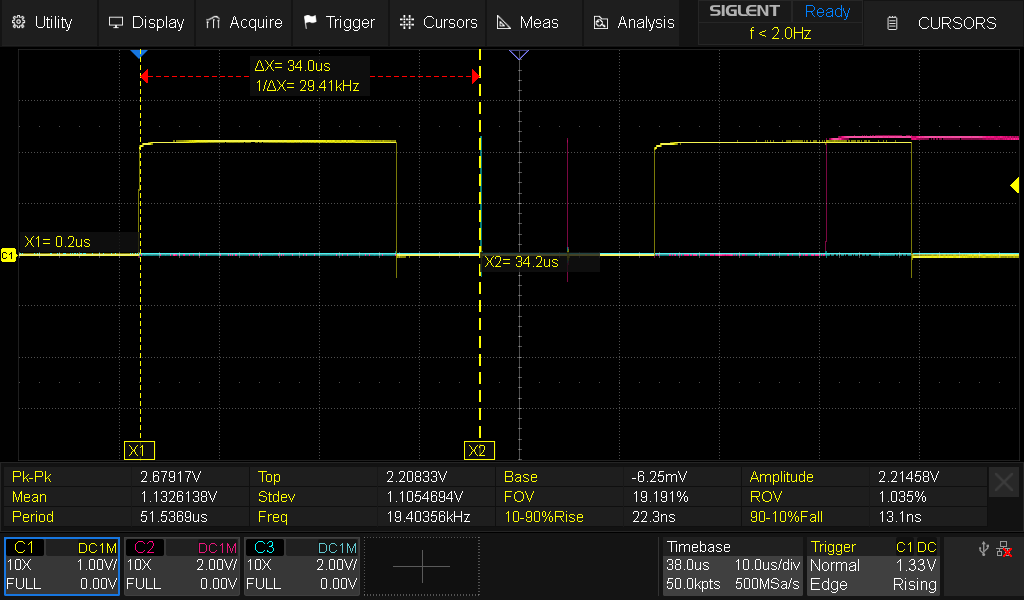
\includegraphics[width=0.75\linewidth]{img/V2_Startup_Jitters_02.png}\\[0.5ex]
  {\small (b) 10\,$\mu$s/div}
  \caption{Start-up of the V2 HVPS controller's three-phase output at a 19.4\,kHz setting (oscilloscope channels C1--C3), one for each phase output from the controller.
    (a) A stray pulse appears about 578\,$\mu$s before the waveform starts. (b) The first periods of the waveform with startup jitter spikes.}
  \label{fig:v2-jitter}
\end{figure}
\todo{Describe what each trace shows and why it saturates the transformer}

Shortly after the inception of the HVPS controller upgrade project, the new Limiter bias supply design project was initiated. Mirroring the HVPS controller, the Limiter supply requires a single-phase pulse-width-modulated (PWM) control signal, with a complementary signal and dead-time insertion, at 100\,kHz. The Limiter currently has one electrode, and may have up to three, each biased independently: each controller output phase (for example U/UN) drives one electrode, and each electrode can follow its own duty-cycle waveform. Each iteration of the HVPS controller and the PFM-G474 controller included peripherals and firmware capable of encoding supply demand signals in either frequency or duty cycle.

The latecomer to the applications of this controller is the Transrex power supplies. In 2025, the Transrex (or XREX) power supplies were commissioned in the WHAM lab to provide up to 20\,kA of current over the course of 30\,s to the WHAM central coils, allowing a variable mirror ratio between the WHAM end and center fields. The commissioning of these supplies was fast-tracked due to the quenching of the WHAM high-temperature superconducting (HTS) coils earlier that same year. 

In the fast-tracked iteration of the Transrex control project, Transrex demand is modulated by an analog voltage driven by the NI CompactRIO (cRIO) in the electron cyclotron heating (ECH) rack, and the only fault monitored for control integrity is the Transrex internal overcurrent fault, which shuts down the faulted supply in a hard stop with no compensation from the other operating supplies. An STM32F4 Nucleo board was originally intended to control the Transrex supplies via I\textsuperscript{2}C communication and DAC output of a linear demand signal to an internal Transrex interface board; however, this project was scrapped when microcontroller lockups were observed in the development stage, owing to the inability of this design to remain galvanically isolated from the high-power switching hardware inside of each Transrex. Each of these issues is addressed in the PFM-G474 controller (PFM-Controller V4 board).

\section{System at a glance}
\label{sec:glance}

Control of WHAM H-Bridge power supplies and Transrex supplies requires low-latency communication with and control of each supply, including detecting supply faults or off-normal shot behavior. In addition, waveform outputs are calculated locally at the controller based on a series of time and demand setpoints sent over network-serial communication from the operator via Labview to the controller being programmed. Figure~\ref{fig:system} shows the path from an operator to a power supply. 

\begin{figure}[H]
  \centering
  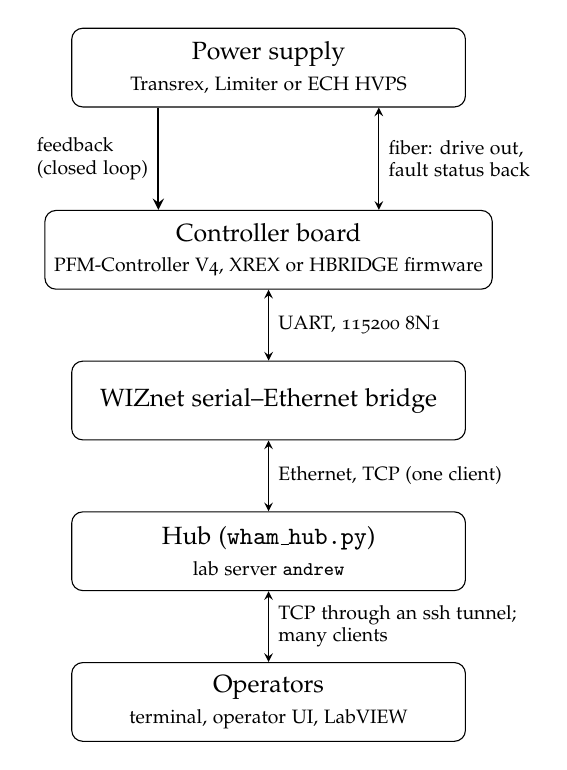
\begin{tikzpicture}[
      node distance=9mm,
      >=stealth,
      box/.style={draw, rounded corners, align=center, minimum width=50mm, minimum height=10mm, font=\small},
      lab/.style={font=\scriptsize, align=left}]
    \node[box] (sup) {Power supply\\ {\scriptsize Transrex, Limiter or ECH HVPS}};
    \node[box, below=13mm of sup] (ctl) {Controller board\\ {\scriptsize PFM-Controller V4, XREX or HBRIDGE firmware}};
    \node[box, below=of ctl] (wiz) {WIZnet serial--Ethernet bridge};
    \node[box, below=of wiz] (hub) {Hub (\texttt{wham\_hub.py})\\ {\scriptsize lab server \texttt{andrew}}};
    \node[box, below=of hub] (cli) {Operators\\ {\scriptsize terminal, operator UI, LabVIEW}};
    % supply <-> controller: drive out and fault status back over fiber; feedback for closed loop
    \draw[<->] ([xshift=14mm]ctl.north) -- node[lab, right]{fiber: drive out,\\ fault status back} ([xshift=14mm]sup.south);
    \draw[->, thick] ([xshift=-14mm]sup.south) -- node[lab, left]{feedback\\ (closed loop)} ([xshift=-14mm]ctl.north);
    \draw[<->] (ctl) -- node[lab, right]{UART, 115200 8N1} (wiz);
    \draw[<->] (wiz) -- node[lab, right]{Ethernet, TCP (one client)} (hub);
    \draw[<->] (hub) -- node[lab, right]{TCP through an ssh tunnel;\\ many clients} (cli);
  \end{tikzpicture}
  \caption{System at a glance. The controller drives the supply and reads its fault status over fiber. In closed-loop operation it
    also reads the supply's output back as feedback (XREX: the unit-current frequency over fiber; HBRIDGE: an analog voltage into
    the controller's ADC). Each board's serial link is shared through one hub on the lab server.}
  \label{fig:system}
\end{figure}

As shown in the system at a glance diagram, real-time communication with the power supply (Transrex, Limiter, HVPS) is only local and with the PFM-Controller (excluding any communication charging supplies, or additional monitoring of the Transrex supplies by Labview - more on that later). Demand signal out of the controller and fault monitoring into the controller is always over Versatile Link fiber optic receivers, transmitters, and cables, though in varying numbers and configurations for each system. 

For closed-loop control\footnote{Not yet commissioned or used in the lab as of Nov 19, 2026}, two configurations are used: For HBRIDGE supplies, ADC inputs are slotted to be used for feedback signal measurement and receive BNC cables; for Transrex supplies, 4-independent fiber optic inputs are configured for PFM measurement and on-board voltage-to-frequency conversion.

Moving further from the supply and controller itself, the PFM Controller board uses UART2 in conjunction with a WIZnet serial-Ethernet bridge and ethernet-to-fiber optic converter to integrate and communicate with the WHAM lab network.\footnote{The specific WIZnet serial-Ethernet board we use is the WIZnet WIZ505SR-RP. Selected based on their \textbf{ease of setup} and \textbf{low price}, they have turned out to mostly be pieces of \textasteriskcentered\textasteriskcentered\textasteriskcentered\textasteriskcentered. I recommend replacing them in the future.}

Because the WIZnet bridge only accepts a single TCP connection at a time, each controller is served by its own instance of the WHAM hub, a small Python service on the lab server \texttt{andrew} that holds that one connection and shares it with any number of users. Operators reach the hub through LabVIEW, the operator UI, or a terminal; Section~\ref{sec:host} describes the hub and when to use each method.

Figure~\ref{fig:states} shows the states, common to both controller firmware configurations.

\begin{figure}[H]
  \centering
  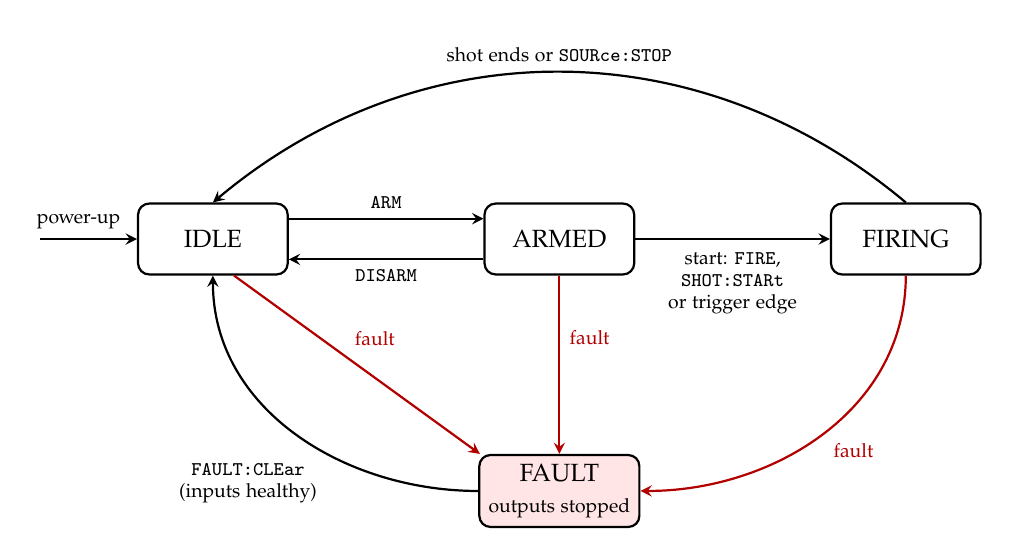
\begin{tikzpicture}[
      >=stealth, thick,
      st/.style={draw, rounded corners, minimum width=19mm, minimum height=9mm, align=center, font=\small},
      lab/.style={font=\scriptsize, align=center}]
    \node[st] (idle)   at (0,0)    {IDLE};
    \node[st] (armed)  at (4.4,0)  {ARMED};
    \node[st] (firing) at (8.8,0)  {FIRING};
    \node[st, fill=red!10] (fault) at (4.4,-3.2) {FAULT\\ {\scriptsize outputs stopped}};
    % power-up
    \draw[->] (-2.2,0) -- node[lab, above, pos=0.4]{power-up} (idle.west);
    % normal cycle
    \draw[->] (idle.15) -- node[lab, above]{\texttt{ARM}} (armed.165);
    \draw[->] (armed.195) -- node[lab, below]{\texttt{DISARM}} (idle.345);
    \draw[->] (armed) -- node[lab, below=1pt]{start: \texttt{FIRE},\\ \texttt{SHOT:STARt}\\ or trigger edge} (firing);
    \draw[->] (firing.north) to[out=140, in=40] node[lab, above]{shot ends or \texttt{SOURce:STOP}} (idle.north);
    % faults
    \draw[->, red!70!black] (idle.300) -- node[lab, above right, pos=0.45]{fault} (fault.155);
    \draw[->, red!70!black] (armed.south) -- node[lab, right, pos=0.35]{fault} (fault.north);
    \draw[->, red!70!black] (firing.south) to[out=-90, in=0] node[lab, below right]{fault} (fault.east);
    % clear
    \draw[->] (fault.west) to[out=180, in=-90] node[lab, below left, pos=0.4]{\texttt{FAULT:CLEar}\\ (inputs healthy)} (idle.south);
  \end{tikzpicture}
  \caption{Operating states of the controller (generic; both products). A shot can start only from ARMED, and every shot needs a new
    \texttt{ARM}. A fault in any state stops the outputs and latches FAULT until \texttt{FAULT:CLEar} finds the fault inputs healthy.}
  \label{fig:states}
\end{figure}

The state machine is the same on both controllers. A controller boots into IDLE (or straight into FAULT if one of its fault inputs is already tripped), where it can be configured and programmed but will not drive anything. \texttt{ARM} only succeeds once the controller is ready: no latched fault, at least one output enabled, and on XREX, the enable and contactor permissives satisfied. What each product does when a fault trips differs, and is described in Sections~\ref{sec:fw-hbridge} and~\ref{sec:fw-xrex}.

\medskip\noindent\textbf{A shot, start to finish.} Putting the pieces together, a typical shot looks like this:
\begin{enumerate}
  \item The operator connects to the controller's hub, checks \texttt{*IDN?} to make sure it is the right board, and checks \texttt{STATE?} for IDLE.
  \item The operator uploads the shot as a series of time and demand setpoints (HBRIDGE: \texttt{SHOT:*}; XREX: \texttt{SHOT:TIMing} and \texttt{SHOT:CURRent}) and reads it back.
  \item \texttt{ARM}, then \texttt{FIRE}, \texttt{SHOT:STARt}, or the external trigger.
  \item The controller calculates the waveform locally, one switching period at a time, drives the supply over fiber, and watches the fault inputs the whole time; in closed loop, it also corrects the output from the feedback signal.
  \item When the shot ends, the controller returns to IDLE, and the hub's log holds a record of everything that was sent.
\end{enumerate}
The full procedures are in Sections~\ref{sec:hbridge-shot} and~\ref{sec:xrex-shot}.

\medskip\noindent\textbf{What the controller does and does not protect.} Protection is layered. The fastest layer is in hardware: a fault on the HRTIM fault input (PC10) disables the outputs in silicon, without any firmware involved. Next, the firmware watches the supply's fault inputs (the gate-driver status lines on HBRIDGE; water, temperature, Enerpro and overcurrent on XREX) and latches FAULT the moment one trips. Last, the interlocks decide whether a shot is allowed to start at all (on XREX, the external enable and each channel's enable and contactor). None of this replaces the facility's own interlocks or the emergency stop: the E-stop is meant to be completely independent of the controller's software, and the controller has no E-stop command. Do not use a typed command as a substitute for it.
\todo{Name the facility interlocks and the E-stop path for each supply}

\medskip\noindent\textbf{Which controller drives which supply.} Every controller is the same PFM-Controller V4 board; what makes it an HBRIDGE or an XREX controller is the firmware image flashed onto it, and an HBRIDGE controller is told at runtime whether it is driving the Limiter or the ECH HVPS (\texttt{CONFig:MODE}). Table~\ref{tab:supplies} summarizes how each supply is driven. The two H-bridge supplies differ in what carries the demand: the Limiter holds its carrier frequency fixed and varies duty cycle, one output per electrode, while the HVPS holds duty near 50\,\% and varies frequency across all three phases. The Transrex controller drives four independent channels, one per supply, each with its own demand frequency and its own fiber feedback.

\begin{table}[H]
  \centering
  \begin{tabular}{L{0.75in} L{1.0in} L{0.9in} L{1.0in} L{0.85in}}
    \hline
    \textbf{Supply} & \textbf{Controller (firmware, mode)} & \textbf{Outputs used} & \textbf{Demand encoded as} & \textbf{Feedback (closed loop)} \\
    \hline
    Limiter & LMTR-CTRL (HBRIDGE, \code{LIMiter}) & U today (V, W for future electrodes) & duty, 5--95\,\%, on a 75--125\,kHz carrier
      & analog voltage $\to$ ADC \\
    ECH HVPS & ECH-HVPS (HBRIDGE, \code{HVPS}) & U, V, W (three-phase) & frequency, 10--30\,kHz, duty 40--60\,\% & analog voltage $\to$ ADC \\
    Transrex $\times$4 & XREX-CTRL (XREX) & 4 channels, one per supply & frequency, 3--150\,kHz & unit-current frequency over fiber \\
    \hline
  \end{tabular}
  \caption{How each supply is driven. Limits are the firmware's own (\texttt{ctrlr\_config.h} in each product).}
  \label{tab:supplies}
\end{table}

Serial numbers, network addresses, hub ports and the current state of each board (installed or on the bench) change over the life of the project, so they are kept in \texttt{host/devices.csv} and \texttt{docs/bench\_devices.md} rather than in this document. As of November 2026, the ECH-HVPS controller is installed in its supply, and the Limiter and Transrex controllers are on the bench.

% ======================================================================
\part{System description}

\section{Hardware}
\label{sec:hardware}

\subsection{Controller PCB (PFM-Controller V4)}
\label{sec:pcb}

The PFM Controller is based around an STM32G474QET6, a micro-control unit (MCU) chip from ST Microelectronics. This MCU features an onboard clock at 170 MHz and several useful peripherals for this application:

\begin{itemize}
  \item \textbf{High-Resolution Timer (HRTIM1):} six timing units, A--F, plus a master timer, all clocked at 170\,MHz (one count is 5.88\,ns). Every drive signal comes from here, each as an output and its complement with hardware dead-time insertion between them (default 100\,ns, set with \texttt{CONFig:DEADtime}). On HBRIDGE, units A--C drive phases U/UN (PA8/PA9), V/VN (PA10/PA11) and W/WN (PB12/PB13) and are reset by the master timer at 0, 1/3 and 2/3 of each period, which keeps the phases locked together; the master timer's period interrupt loads the next period's frequency and duty from the shot. On XREX, each of the four channels runs on its own unit with its own period, updated at that unit's own roll-over, so the four frequencies are fully independent. Further units are routed to PB14/15, PC8/9 and PC6/7.
  \item \textbf{HRTIM fault input (FLT6, PC10):} a hardware fault input that forces the outputs safe in silicon the moment it trips, with no firmware in the path.
  \item \textbf{General-purpose timers TIM2--TIM5:} input capture on the six fiber inputs (PFM\_Input 1--6: PA15, PD4, PB2, PC12, PB4, PD12), with DMA (DMA1 channels 1--6) moving each edge's timestamp into memory. On XREX this measures the unit-current feedback frequency from each Transrex; on HBRIDGE it is used to check a shot's actual output on the bench (\texttt{PFMIN:CAPTURE}).
  \item \textbf{ADC1, TIM6 and DMA (HBRIDGE):} TIM6 triggers a scan of six analog inputs (PA0, PA1, PC0, PB0, PC1, PB1) plus the internal reference; DMA (DMA2 channel 1) fills a circular buffer, and each completed block is one closed-loop control tick (10\,kHz by default, \texttt{CONFig:PIDRate}).
  \item \textbf{DAC1 (PA4, PA5, HBRIDGE):} drives a test voltage back into the ADC inputs for hardware-in-the-loop testing of the closed loop.
  \item \textbf{TIM20 (PG0, HBRIDGE):} channel 1's complementary output makes the 50\,\% square wave for the capacitor-bank charger (\texttt{CHARGE:FREQuency}).
  \item \textbf{QUADSPI:} talks to the external W25Q128 flash (16\,MB; PE12--PE15, PB10, PB11), which holds the saved profiles and the board's identity (serial number and label).
  \item \textbf{USART2 (PA2/PA3):} the command link, 115200 8N1, interrupt-driven receive; wired to the WIZnet bridge and the USB-serial header.
  \item \textbf{EXTI (external interrupts):} turns pin edges into interrupts. On HBRIDGE, the 12 gate-driver status inputs (PE0--PE11) interrupt on both edges so a fault stops the outputs immediately, and PF15 interrupts on a rising edge for the external trigger.
  \item \textbf{Dual-bank flash and option bytes:} the 512\,KB of flash is split into two banks, so a new firmware image can be written to the bank that is not running and then swapped in (\texttt{FWUPdate:*}), with the old image kept for rollback.
  \item \textbf{TIM16/TIM17 and DMA (DMA1 channels 7 and 8):} turn the serial-activity LEDs off after a short pulse with no CPU involvement.
  \item \textbf{GPIO:} the remaining inputs and outputs, among them the XREX external-enable interlock (PF13), the XREX per-channel enable and contactor outputs (PG0--PG7), and the front-panel status LEDs.
\end{itemize}
\noindent\src{firmware/*/src/bsp/stm32g4/ (hrtim.c, pfm\_input.c, adc.c, charge\_out.c, qspi\_test.c, led\_indicators.c); pin\_mapping\_v4.csv}


\begin{itemize}
  \item MCU: STM32G474QET6, Cortex-M4F at 170\,MHz, 512\,KB flash in two banks, 128\,KB RAM, LQFP128.
  \item Gate-driver / fault inputs: PE0--PE11 (GateDriverStatus\_01--12), no pull resistors.
  \item Debug: SWD on PA13/PA14; NRST (pin 21, labeled PG10); BOOT0 on PB8.
  \item Front-panel LEDs: PD2, PD3, PF14, PF2, PC3, PC2 (serial activity and the four states; verify which pin is which).
  \item Board revisions: \file{hardware/PFM-Controller_V4} (current), \file{PFM-Controller_V4_Rev2}, \file{HVPS_Controller_V3} (previous).
    \code{HW\_BOARD\_REV} in firmware is a placeholder (\code{"REVA"}).
  \item \todo{Power tree, input voltage, regulators and current budget}
  \item \todo{Design rationale for the V4 layout (fiber transceivers, isolation, connectors)}
  \item \todo{Board photo with connectors labeled}
\end{itemize}
\noindent\src{firmware/*/docs/pin\_mapping\_v4.csv; hardware/README.md; handoff/02 \S2.1}

The WHAM-PFMG474 is based around the STM32G474QET6 microcontroller unit from ST Microelectronics. This MCU was selected for its high clock speed (170MHz) High-Resolution Timer (HRTIM) peripherals, and large GPIO pin count. 

\subsection{Enclosure and other contents}
\label{sec:box}
\begin{figure}[H]
  \centering
  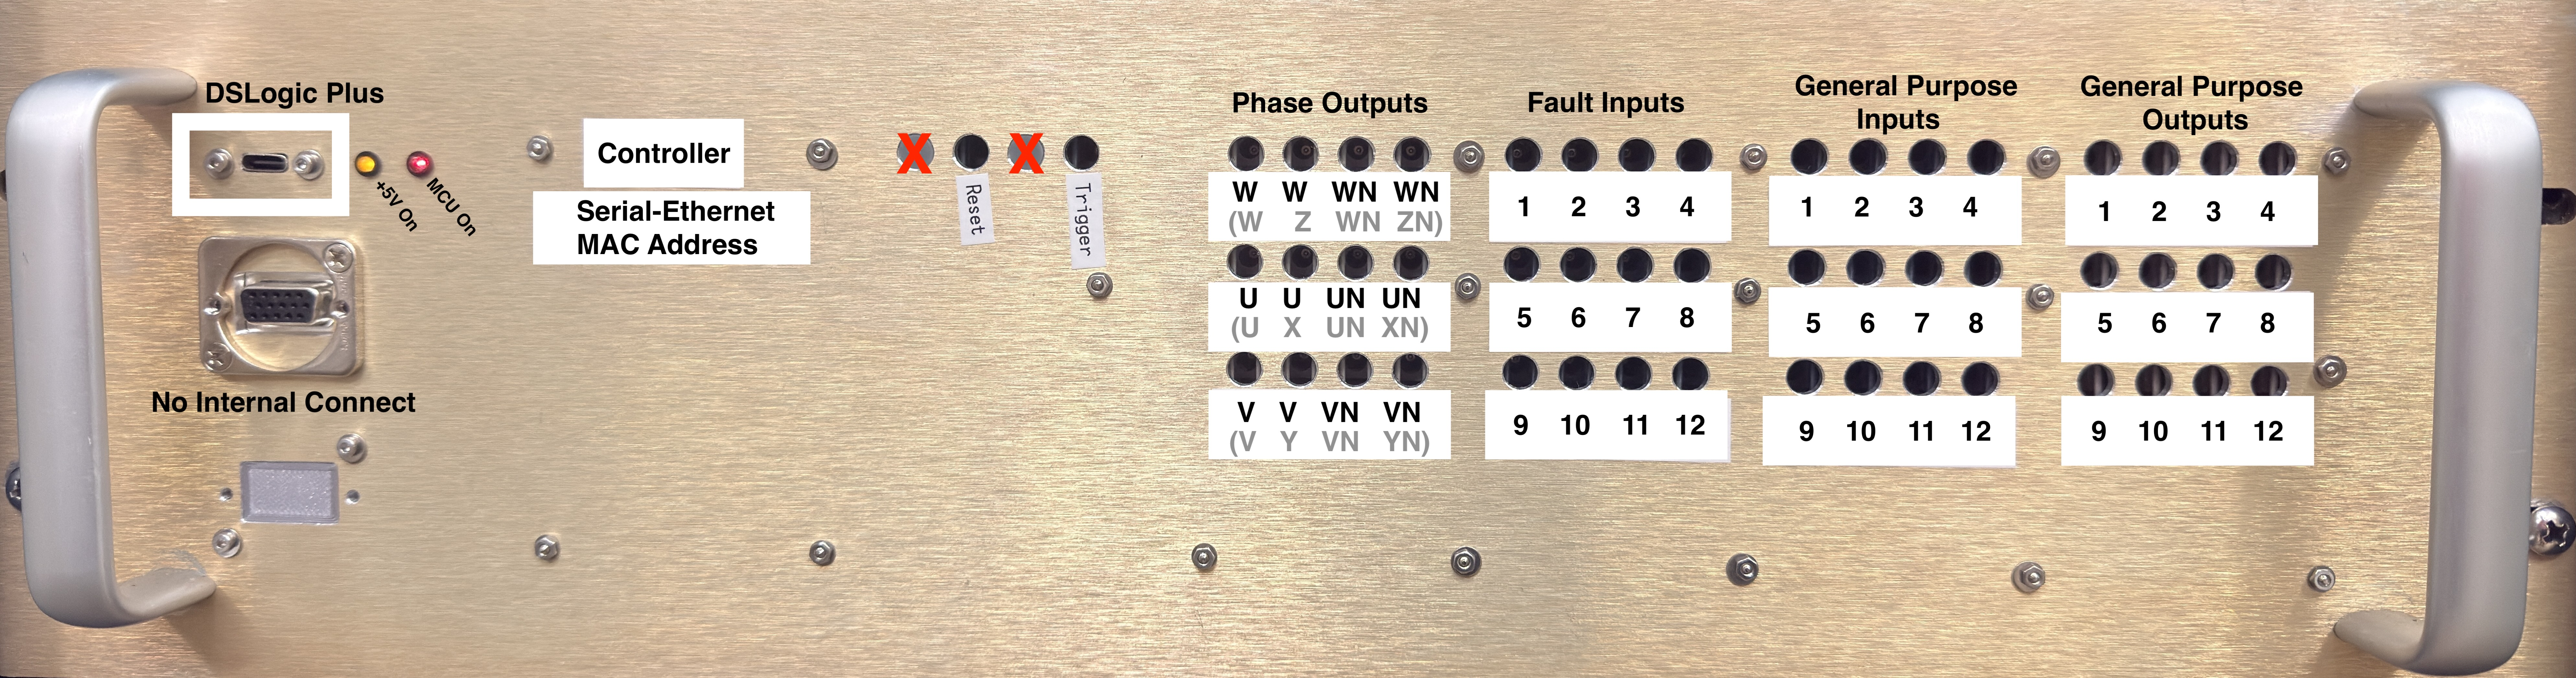
\includegraphics[width=\linewidth]{img/front-panel_01_redacted.JPG}
  \caption{Front panel of the controller enclosure, annotated: phase outputs, fault inputs, general-purpose inputs and
    outputs, the DSLogic port and the status LEDs. Fiber inputs marked with a red X are not wired internally.}
  \label{fig:front-panel-xrex}
\end{figure}
\begin{itemize}
  \item Fill in one table per installation (columns below). Known rows are pre-filled.
  \item \todo{Complete the enclosure inventory for each installation}
\end{itemize}
\begin{center}
\begin{longtable}{L{0.85in} L{0.75in} L{0.85in} L{0.75in} L{1.2in}}
  \hline
  \textbf{Item} & \textbf{Part / model} & \textbf{Function} & \textbf{Connects to} & \textbf{Notes} \\
  \hline
  \endhead
  Controller PCB & PFM-Controller V4 & MCU, drive and I/O & everything & NRST pull-up required (\S\ref{sec:hwmods}) \\
  Serial-Ethernet bridge & WIZnet WIZ5XX\-SR-RP, fw 1.0.5 & UART to TCP (server, port 5000) & USART2, lab network & one client only; 8N1 fixed \\
  USB-serial adapter & CH340-based & bench serial link & USART2 header & port names change on replug \\
  Fiber transmitters / receivers & & drive, feedback, fault signals & supply & \todo{Fiber transceivers: type, count, wavelength} \\
  Power entry / supply & & board power & & \todo{Power entry: model and rating} \\
  Connectors, front panel & & & & \todo{Connectors and front panel: list} \\
  Daughter board & \file{hvps_v3_ix4340_daughter_board} & & & \todo{Daughter board: role, if fitted} \\
  Cabling & & & & \todo{Cabling: harness list} \\
  Enclosure, grounding & & & & \todo{Enclosure and grounding: details} \\
  \hline
\end{longtable}
\end{center}
\src{docs/bench\_devices.md; hardware/PFM-Controller\_V4/}

\subsection{Signals and I/O per product}
\label{sec:signals}
\begin{itemize}
  \item XREX: per channel XR1--XR4: DRIVE (demand, PFM out), FEEDBACK (unit current, PFM in), ENA\_OUT (PG0--PG3),
    CONTACT\_OUT (PG4--PG7), water/temp/Enerpro faults (on PE0--PE11), OCP (PF4, PF5, PF8, PF12, polled).
    System-wide: PF13 external enable, PF15 external trigger, PC10 hardware fault; bench-only diagnostic outputs.
    \src{former XREX SOP, ``Controller I/O'' section (lines 807--968); pin\_mapping\_v4.csv ``XREX Pin Name'' column}
  \item HBRIDGE: U/UN, V/VN, W/WN (HRTIM A--C); GDS 01--12 (PE0--PE11); PC10 hardware fault; PF15 trigger; PG0 CHARGE
    (TIM20 CH1N); ADC feedback (default U = PA0, V = PA1, W = PB0); DAC PA4/PA5. \src{firmware/hbridge/AGENTS.md}
  \item \todo{One signal table per product: signal, pin, direction, level and polarity, connector, what it connects to}
\end{itemize}

\subsection{Required hardware modifications}
\label{sec:hwmods}
\begin{itemize}
  \item NRST pull-up: 5.1\,k$\Omega$ from NRST to 3.3\,V on every board. Without it the board can stay in reset after a firmware
    swap or power-up (NRST measured 1.6\,V). Never tie NRST hard to 3.3\,V; never fit a pull-down. Source of the load not found.
    \src{former XREX SOP \S3.3 (lines 189--279); xrex changelog 2026-09-28/29; handoff/06 \S6.1}
  \item BOOT0 (PB8) floats on some boards: either a 10\,k$\Omega$ pull-down or option bit \code{nSWBOOT0 = 0}. The former
    simulator board (now LMTR-CTRL) was set to \code{FLASH\_OPTR = 0xBBEFF8AA} (recorded 2026-09-28; re-read with \code{DIAGnostic:OPTBytes?}). \src{handoff/06 \S6.2}
  \item Unwired fault inputs read as faults (no pull resistors): a bench board boots in \code{FAULT}. \src{handoff/06 \S6.4}
  \item ST-Link wiring with the pull-up fitted: SWDIO, SWCLK, GND, 3V3 only; NRST wire off.
  \item \todo{Record of which boards have the modification fitted, and how (photo)}
\end{itemize}

% ----------------------------------------------------------------------
\section{Firmware}
\label{sec:firmware}

\subsection{Common platform}
\label{sec:platform}
\begin{itemize}
  \item Bare metal, C11, ST HAL; built with STM32CubeIDE's toolchain (arm-none-eabi-gcc 13.3) through \code{python/wham\_build.py}.
  \item Layered source: \file{Core/} (CubeMX only), \file{src/config}, \file{src/drivers} (interfaces), \file{src/bsp/stm32g4}
    (the only hardware code), \file{src/middleware/scpi}, \file{src/app}; host tests in \file{tests/}; enforced by \code{check\_layout.py}.
  \item Main loop of non-blocking tasks; time-critical work in interrupts (HRTIM per-period, control tick, fault edges, UART).
    Priorities are set deliberately and differ by product. \src{handoff/02 \S2.2; handoff/07 \S7.3}
  \item Operating states \code{IDLE}, \code{ARMED}, \code{FIRING}, \code{FAULT}; every shot needs its own \code{ARM}; faults latch
    until \code{FAULT:CLEar}, which re-checks the inputs.
  \item Command protocol: SCPI style, long/short forms, one-line replies \code{OK ...} / \code{ERR <code> <text>}; strict
    arguments; frozen error codes. \src{firmware/*/docs/scpi\_conventions.md}
  \item Firmware update: dual bank, CRC, swap, rollback; \code{!BOOT} banner; needs \code{IDLE}; refuses the other product's image.
  \item Saved profiles: 8 slots in the W25Q128, recall only on request; XREX region 0--64\,KiB (\code{WSPF}), HBRIDGE 64--320\,KiB
    (\code{HSPF}), identity in the last sectors. Field ids frozen.
  \item Identity: MCU UID, flash UID, provisioned serial \code{WB-NNNN-C} and label; reported, never enforced.
  \item Code shared byte-for-byte between the products, checked by \code{check\_shared.py}.
  \src{handoff/02; firmware/*/AGENTS.md}
\end{itemize}

\subsection{Peripheral usage}
\label{sec:peripherals}
\begin{center}
\begin{longtable}{L{1.1in} L{0.75in} L{2.8in}}
  \hline
  \textbf{Peripheral} & \textbf{Product} & \textbf{Use} \\
  \hline
  \endhead
  HRTIM1 Master + A--F & both & drive outputs; XREX: one unit per channel, own period; HBRIDGE: A--C phase-locked to the Master \\
  HRTIM1 FLT6 (PC10) & both & hardware fault input, outputs forced safe in silicon \\
  TIM2--TIM5 & both & period capture on PFM inputs (XREX feedback; HBRIDGE bench checks, duty meter) \\
  TIM16/17 + DMA1 ch 7/8 & both & LED one-pulse turn-off \\
  TIM20 CH1N (PG0) & HBRIDGE & CHARGE square wave \\
  ADC1 + DMA, timer trigger & HBRIDGE & closed-loop feedback, one control tick per DMA block \\
  DAC (PA4, PA5) & HBRIDGE & hardware-in-the-loop tests \\
  QUADSPI & both & W25Q128: profiles, identity \\
  USART2 & both & command link (115200 8N1) \\
  EXTI lines & both & fault inputs (PE0--PE11), PF15 trigger (HBRIDGE) \\
  CORDIC vector & HBRIDGE & used as a software interrupt for the shot start \\
  Flash dual bank, option bytes & both & firmware update (BFB2) \\
  \hline
\end{longtable}
\end{center}
\src{handoff/02; firmware/*/AGENTS.md}. \todo{Check the table against the current code and add interrupt priorities per product}

\subsection{H-bridge firmware (HBRIDGE)}
\label{sec:fw-hbridge}
\begin{itemize}
  \item Supply mode: \code{CONFig:MODE LIMiter|HVPS}; Limiter 75--125\,kHz, 5--95\,\% duty; HVPS 10--30\,kHz, 40--60\,\%; boot
    mode \code{NONE}; changing mode discards the shot.
  \item Phases U at 0, V at 1/3, W at 2/3 of a period (Master resets). The HVPS needs this three-phase spacing; in Limiter mode it is
    only carried over from the HVPS, since the Limiter needs no particular phase relationship between its electrodes; output SET on CMP3 (pulse-collision fix, 2026-09-09);
    each phase connected at its own reset on start (2026-09-04).
  \item Dead time: one value for all phases, 50--3000\,ns, default 100\,ns, 5.88\,ns steps (\code{CONFig:DEADtime}).
  \item Shot engine: up to 500 setpoints, 1\,s, linear interpolation per period, optional duty per phase; 0\,Hz = output-off gap.
  \item Closed loop: one loop per phase (Limiter), one frequency loop (HVPS); ADC feedback, plant-model feedforward plus PID;
    overvoltage and feedback faults; \code{PID:LOOPMODE} per phase.
  \item Protection: 12 GDS inputs, one fault type, immediate force-stop; per-input enable, nicknames, runtime polarity flip.
  \item External trigger: PF15 rising edge while \code{ARMED}; on by default at boot; interrupt-driven.
  \item CHARGE output: 50\,\% square wave on PG0, independent of faults.
  \item What a profile stores: settings, tables, GDS configuration, dead time, phases; not run state, CHARGE, trigger, bypass, DAC, simulation.
  \src{firmware/hbridge/AGENTS.md; firmware/hbridge/docs/saved\_profiles.md; handoff/02 \S2.4}
  \item \todo{Expand into prose with one timing diagram of a three-phase period and one of a gap}
\end{itemize}

\subsection{Transrex firmware (XREX)}
\label{sec:fw-xrex}
\begin{itemize}
  \item Four independent channels, each on its own HRTIM unit, updated at its own roll-over (``Possibility 3'').
    \src{firmware/xrex/docs/Transrex/hrtim\_divergent\_period\_timing.pdf (cite, do not reproduce)}
  \item Fixed-rate PID (default 1\,kHz, \code{CONFig:PIDRate}), decoupled from the carriers; output 3--150\,kHz.
  \item Shots: ramp up, flat top, ramp down (\code{SHOT:TIMing}) to a demand current per channel (\code{SHOT:CURRent});
    amps converted to hertz by a linear placeholder calibration.
  \item Faults: water, temperature, Enerpro, overcurrent per channel; general fault; ramp-down of surviving channels;
    overcurrent step-down by $100/N$\,\%.
  \item Interlocks: PF13 external enable; ENA\_OUT and CONTACT\_OUT required for \code{ARM}; PF15 trigger (polled).
  \item Simulator build target: a second board imitates four Transrex supplies.
  \item Legacy table mode (\code{TABle:*}, \code{FIRE}): bench fallback only.
  \item Calibration placeholders (not yet measured): maximum current per channel, turn-on and maximum frequency, amps-to-Hz,
    slew limit, fault ramp time, PID gains. \src{handoff/08 \S8.2}
  \src{firmware/xrex/AGENTS.md; firmware/xrex/docs/Transrex/Transrex\_Controls\_Upgrade (1).pdf (cite only)}
\end{itemize}

\subsection{Settled design decisions}
\label{sec:decisions}
\begin{itemize}
  \item Summarize as a table: decision, reason, date. Source: \file{handoff/03_design_decisions.md}.
  \item \todo{Select which decisions belong in the SOP}
\end{itemize}

% ----------------------------------------------------------------------
\section{Host software and interfacing}
\label{sec:host}
\subsection{The WHAM hub}
\label{sec:hub}
The WIZnet bridge only accepts a single TCP connection at a time, which is fine for one engineer at a bench but not for a lab where LabVIEW, an operator, and whoever is debugging the controller may all need it at once. To get around this, each controller is served by its own instance of the WHAM hub (\texttt{host/wham\_hub.py}), a small Python service running on the lab server \texttt{andrew}. The hub is the only client of the controller's bridge, and it shares that one connection with any number of users, each controller on its own port. Commands are passed to the controller one at a time, and each reply is returned to whoever sent the command. 

Additionally, the hub does a few jobs that make the system safer and easier to debug: it asks the board who it is (\texttt{*IDN?} and \texttt{SYS:ID?}) when it connects and after every reboot, and can refuse to forward commands to the wrong board; it logs every line sent and received, with the board's serial number, to a daily log file; it notices a dead link and reconnects on its own; and it announces dangerous commands (anything that arms, fires, or switches off a protection) to everyone else connected. There is currently no lock or authentication, so anyone who can reach a hub's port can send any command, including \texttt{ARM} and \texttt{FIRE}. The hub ports for each controller are listed in \texttt{docs/bench\_devices.md}.

\subsection{Connecting to a hub}
\label{sec:hub-connect}
There are three ways to connect to a hub, depending on who you are and what you are doing. From outside the lab network, each method first needs an ssh tunnel to \texttt{andrew}, which makes the hub's port appear on your own computer.
\begin{itemize}
  \item \textbf{LabVIEW} connects in quiet mode (\texttt{@quiet} as its first line), so it sees only the replies to its own commands. This is the method for running shots as part of WHAM operation (\texttt{docs/labview\_hub\_guide.md}).
  \item \textbf{The operator UI} (\texttt{host/operator\_ui/}) is a local web page for operators who would rather click than type: it connects to a hub, confirms dangerous commands with a dialog, builds and reads back shots, and can record shot data (\texttt{docs/operator\_ui\_guide.md}).
  \item \textbf{A terminal} (\texttt{net\_client.py}) gives raw SCPI access and shows what everyone else on that controller is sending. This is the engineer's method: debugging, bench tests, and firmware updates (\texttt{fw\_update.py} runs through the hub the same way) (\texttt{docs/operator\_hub\_connection.md}).
\end{itemize}
On the bench, a controller can also be reached directly through its USB-serial port, bypassing the network and the hub entirely; this is for bring-up and recovery only. Step-by-step instructions for every method are in Appendix~\ref{app:connect}.

\subsection{Other host-side pieces}
\begin{itemize}
  \item WIZnet bridge: one TCP client, fixed 8N1 (so the ROM bootloader cannot be used over the network), drops characters in long replies.
  \item Python tools in \file{firmware/<product>/python/}: build, update, shot tests, reports.
  \item Device registry and provisioning: \file{host/devices.csv}, \file{host/provision_board.py}.
  \item \todo{Network diagram with the lab server, bridges and operator computers}
\end{itemize}
\noindent\src{host/README.md; handoff/02 \S2.7}

% ======================================================================
\part{Procedures}

\note{Every procedure uses the same headings. Every command named in this document was checked against the product's
command table on 2026-11-18; the full syntax and replies are in \file{command_reference.md}.}

\section{Set up a workstation}
\label{sec:workstation}
\begin{procedure}
  \pitem{Purpose} Install what is needed to build firmware and reach the boards.
  \pitem{Who} Maintaining engineer.
  \pitem{Prerequisites} \todo{Supported operating systems; accounts needed}
  \pitem{Steps}
    \begin{enumerate}
      \item STM32CubeIDE (toolchain on \code{PATH}); Python~3 with pyserial, numpy, matplotlib; git; host C compiler.
      \item ST-Link driver and openocd (or st-flash); logic-analyzer software.
      \item ssh key access to \code{andrew}. \todo{Who grants access}
      \item Clone the repository; run \code{python3 python/wham\_build.py} once in each product folder.
    \end{enumerate}
  \pitem{Afterwards} The build ends with \code{[done]} and an image in \file{build/}.
  \src{former XREX SOP, Prerequisites (lines 145--188); handoff/04 \S4.1}
\end{procedure}

\section{Connect to and identify a controller}
\label{sec:connect}
\begin{procedure}
  \pitem{Purpose} Open a session with the right board.
  \pitem{Who} Anyone authorized to use the board.
  \pitem{Steps}
    \begin{enumerate}
      \item Open the tunnel: \code{ssh -f -N -L <local>:127.0.0.1:<hub port> andrew} (hub ports in \file{docs/bench_devices.md}; choose a free local port).
      \item Connect: \code{python3 firmware/<product>/python/net\_client.py --port <local> --name <you>}.
      \item \cl{*IDN?}{OK <product> <rev> <version> <commit> SN=WB-... UID=...}
      \item \cl{STATE?}{OK IDLE} (or \code{OK FAULT ...} on an unwired bench board).
      \item \cl{!hub status}{\# hub ... connected=1 ...}
    \end{enumerate}
  \pitem{If the reply differs} Wrong product or serial: disconnect at once. No reply: check the hub (\code{connected=}),
    then ping the bridge from \code{andrew}.
  \pitem{Direct USB-serial} 115200 8N1; identify by \code{*IDN?}; wait about 1.5\,s after opening the port.
  \src{handoff/05 \S5.2; operators\_guide.md \S5}
\end{procedure}

\section{Build the firmware}
\label{sec:build}
\begin{procedure}
  \pitem{Steps}
    \begin{enumerate}
      \item Commit or stash unrelated changes (an uncommitted tree makes the version read \code{-dirty}).
      \item \code{cd firmware/<product>} then \code{python3 python/wham\_build.py} (XREX simulator: \code{--target simulator}).
      \item Check the output: tests pass, zero warnings, image in \file{build/}.
    \end{enumerate}
  \pitem{Never} flash an image from a bare \code{make}.
  \src{former XREX SOP, Build (lines 280--302); handoff/04 \S4.2}
\end{procedure}

\section{Flash and update firmware}
\label{sec:flash}
\caution{Ask the owner before every flash. State the board (serial), the image (commit) and why.}

\subsection{In-application update over the network (normal)}
\label{sec:fwupdate}
\begin{procedure}
  \pitem{Prerequisites} Owner OK; board safe; image built (\S\ref{sec:build}); board in \code{IDLE}.
  \pitem{Reaching IDLE on a bench board}
    HBRIDGE:\\ \cl{GDS:ENAble 0 0}{OK}\\ \cl{FAULT:CLEar}{OK}\\ \cl{STATE?}{OK IDLE}\\
    XREX:\\ \cl{EXTernal:ENAble 0}{OK}\\ \cl{FAULT:CLEar}{OK}\\ \cl{STATE?}{OK IDLE}\\
    Not on a board connected to a supply without knowing why its interlocks are unsatisfied.
  \pitem{Steps}
    \begin{enumerate}
      \item \code{python3 python/fw\_update.py --url socket://localhost:<port> --yes}
      \item Expect \code{OK VERIFIED CRC=...}, \code{OK SWAPPING}, the \code{!BOOT} banner, then
        \code{[ok] now running <version> <commit> from bank <n>}.
    \end{enumerate}
  \pitem{Afterwards} Verify (\S\ref{sec:verify}). Settings are back at defaults; recall a profile if needed.
  \src{former XREX SOP, Network Firmware Update (lines 366--436); handoff/05 \S5.3}
\end{procedure}

\subsection{Rollback}
\begin{itemize}
  \item \code{python3 python/fw\_update.py --url socket://localhost:<port> --rollback}; the previous image is in the other bank.
  \item \code{fw\_update.py --status} or \cl{FWUPdate:STATus?}{OK BANK=<n> BFB2=<0|1> ...}
\end{itemize}

\subsection{Bootstrap flash over SWD}
\begin{itemize}
  \item For a blank board, a dead serial link, or a change of product.
  \item Wiring: SWDIO, SWCLK, GND, 3V3; NRST wire off; target voltage about 3.3\,V.
  \item openocd: \code{-f interface/stlink.cfg -c "transport select hla\_swd" -f target/stm32g4x.cfg -c "reset\_config none"
    -c "adapter speed 480"}, then \code{program <bin> 0x08000000 verify}, \code{reset run}.
  \item st-flash only when the board runs bank~1 (\code{BANK=1 BFB2=0}).
  \src{former XREX SOP, Bootstrap Flash (lines 303--321); handoff/05 \S5.4}
\end{itemize}

\subsection{Serial ROM-bootloader reflash (bench only)}
\begin{itemize}
  \item \code{wham\_serial\_flash.py} over a direct USB-serial link (\code{BOOT} + stm32flash); not possible through the network bridge (8N1).
  \src{former XREX SOP, Serial Reflash (lines 322--365); firmware/*/docs/serial\_reflash\_guide.md}
\end{itemize}

\subsection{Verify after flashing}
\label{sec:verify}
\begin{itemize}
  \item \code{*IDN?} shows the expected commit (no \code{-dirty} for a release build); \code{STATE?}; \code{DIAGnostic:RSTCause?}.
  \item \todo{Release checklist: which settings and profiles to restore after an update}
  \src{former XREX SOP, Verification (lines 437--458)}
\end{itemize}

\section{Provision a new board}
\label{sec:provision}
\begin{itemize}
  \item Fit and check the NRST pull-up (\S\ref{sec:hwmods}); record the option bytes (\code{DIAGnostic:OPTBytes?}).
  \item Bootstrap flash over SWD; verify.
  \item Assign the serial and label with \file{host/provision_board.py}; registry \file{host/devices.csv}; \code{SYS:SERial} can be written once.
  \item Add the board to \file{docs/bench_devices.md} and a hub config in \file{host/config/}.
  \src{docs/device\_identity\_and\_host\_service.md; host/README.md}
  \item \todo{Labeling and physical inventory steps}
\end{itemize}

\section{Configure and save settings}
\label{sec:profiles}
\begin{itemize}
  \item Read back every setting with its \code{?} query; several setters round or clamp.
  \item \cl{CONFig:PROFile:CATalog?}{OK 1=<label>/<fw> 2=empty ...}
  \item \cl{*SAV <slot> <label>}{OK} (\code{IDLE} only).
  \item Before a recall: \code{CONFig:PROFile:DIFF? <slot>} and show it to the board owner.
  \item \cl{*RCL <slot>}{OK APPLIED=<n> FAILED=0 [GDSOFF=<j>]}; a recall can change the supply mode, phases, dead time, GDS
    polarity and enables: read them back.
  \item Nothing is loaded at boot.
  \src{firmware/hbridge/docs/saved\_profiles.md; handoff/05 \S5.6}
\end{itemize}

\section{Run an HBRIDGE shot}
\label{sec:hbridge-shot}
\caution{Needs the owner's OK. The ECH-HVPS is installed in its supply.}
\begin{procedure}
  \pitem{Prerequisites} Owner OK; identified board; \code{STATE? -> OK IDLE}.
  \pitem{Steps}
    \begin{enumerate}
      \item \cl{CONFig:MODE HVPS}{OK} (or \code{LIMiter}); \code{CONFig:LIMits?}.
      \item Select the phases (\code{IDLE} only). All three are enabled at every boot unless a recalled profile says otherwise.
        Limiter today (one electrode, on U): \cl{PHASe:SELect U}{OK}. HVPS: \cl{PHASe:SELect UVW}{OK}. Check with
        \cl{PHASe:ENAble?}{OK U=1 V=0 W=0} (Limiter).
      \item \code{CONFig:DEADtime?}; \code{EXTernal:TRIGger 0} unless the trigger is wanted.
      \item \cl{SHOT:BEGin}{OK}
      \item \cl{SHOT:STEP 0 20000 50}{OK} (time in $\mu$s, frequency in Hz, duty in \%), one line per setpoint
      \item \cl{SHOT:END}{OK <points> <duration\_us>}
      \item \code{SHOT?} and \code{SHOT:POINt? <i>} to read back.
      \item Optional check: \code{PFMIN:CAPTURE <n>} before firing.
      \item \cl{ARM}{OK}
      \item \cl{FIRE}{OK}; \code{STATE?} shows \code{FIRING}, then \code{IDLE}.
    \end{enumerate}
  \pitem{If the reply differs} \code{ERR 10}: outside the mode's limits; \code{ERR 4}: order or format; \code{ERR 13}: wrong state.
  \pitem{Afterwards} Safe state (\S\ref{sec:shutdown}).
  \pitem{Limiter: adding a second or third electrode (V, W)}
    \begin{itemize}
      \item Each electrode is driven by one phase: U/UN today; V/VN and W/WN are spare.
      \item Wire the new electrode's bridge to the phase's gate-drive pair (V: PA10/PA11; W: PB12/PB13).
      \item Wire that bridge's gate-driver status signals to free GDS inputs, then \code{GDS:ENAble <n> 1} and
        \code{GDS:NICKname <n> <name>} for each.
      \item Closed loop: its feedback goes to the phase's ADC input (defaults: V = PA1, W = PB0; \code{CONFig:FEEDback:CHANnel}
        changes it).
      \item \cl{PHASe:SELect UV}{OK} (or \code{UVW}); upload per-electrode duties with
        \code{SHOT:STEP <t\_us> <hz> <dU> <dV> <dW>} (carrier and time stay shared).
      \item Check the new output with \code{PFMIN:CAPTURE} or a logic analyzer before connecting the electrode.
      \item \code{*SAV} a profile: it stores the phase choice and the GDS configuration.
      \item The phases sit at 0, 1/3 and 2/3 of the period, carried over from the HVPS; the Limiter needs no particular
        relationship (\S\ref{sec:fw-hbridge}).
      \item \todo{Electrode bridge hardware and wiring details for V and W}
    \end{itemize}
  \pitem{Closed-loop runs} Engineer only: \code{PID:LOOPMODE}, \code{TARGet:*}. \todo{Closed-loop run procedure once commissioned}
  \src{handoff/05 \S5.5; firmware/hbridge/docs/operators\_guide.md \S6; docs/labview\_commands.md \S4}
\end{procedure}

\section{Run an XREX shot}
\label{sec:xrex-shot}
\caution{Needs the owner's OK.}
\begin{procedure}
  \pitem{Steps}
    \begin{enumerate}
      \item \code{SOURce:ENAble <ch> 1} for each channel; \code{CHANnel:NICKname} optional.
      \item \cl{SHOT:TIMing <rampUpS> <flatTopS> <rampDownS>}{OK}
      \item \cl{SHOT:CURRent <ch> <amps>}{OK} for each channel
      \item Interlocks: \code{EXTernal:ENAble?}, \code{EXTernal:INPut?}, \code{XREX:CHANnel:STATus? <ch>}.
      \item Optional recording: \code{LOG:ARM <ch> <maxSamples> <decim>}.
      \item \cl{ARM}{OK}
      \item \cl{SHOT:STARt}{OK} (or the PF15 trigger)
      \item After: \code{LOG:DATA?}; \code{SYS:EVLOG?} for the event history.
    \end{enumerate}
  \src{former XREX SOP, ``Program and Fire a Shot Profile'' (lines 522--685) and ``Telemetry'' (lines 686--806);
    firmware/xrex/docs/operators\_guide.md \S6}
  \pitem{Note} Amps are converted with a placeholder calibration (\S\ref{sec:fw-xrex}).
\end{procedure}

\section{Fault response and recovery}
\label{sec:faults}
\begin{itemize}
  \item Read: \code{STATE?}, \code{FAULT?}; HBRIDGE \code{FAULT:SOURces?}, \code{GDS:LAST?}, \code{GDS?}; XREX \code{XREX:CHANnel:STATus? <ch>}.
  \item Decide: real fault, wiring, or an unwired bench input. \todo{Decision tree and who to call}
  \item \code{FAULT:CLEar} re-checks the inputs; it stays in \code{FAULT} if an input is still bad.
  \src{docs/labview\_state\_and\_faults.md; operators\_guide.md \S9}
\end{itemize}

\section{Bench-only procedures}
\label{sec:bench}
\begin{itemize}
  \item Reaching \code{IDLE} on an unwired board (\S\ref{sec:fwupdate}).
  \item \code{DEBUG:FAULT:BYPASS 1|0}: ignore fault inputs on the bench; dangerous.
  \item Legacy \code{TABle:*} / \code{FIRE}. \src{former SOPs, ``Upload and Fire a PFM Table''}
  \item Measuring a shot: \code{pfm\_shot\_test.py}, \code{pfm\_gap\_test.py} (they fire); DSLogic capture (close DSView first).
  \src{handoff/05 \S5.5}
\end{itemize}

\section{Commissioning and calibration on a real supply}
\label{sec:commissioning}
\note{Not yet performed for either product.}
\begin{itemize}
  \item XREX: measure each supply's current at maximum frequency (\code{CONFig:MAXCURRent}); confirm turn-on and maximum
    frequency; replace the linear amps-to-Hz map; set slew and fault ramp time; tune PID (start with low Ki: jitter grows
    with Ki; sweep Ki 25--250).
  \item HBRIDGE: feedback calibration (\code{CONFig:FEEDback:*}), \code{CONFig:MAXVolts}, plant model, PID per phase;
    dead time on the real bridge.
  \item \todo{Commissioning procedure, acceptance criteria and sign-off}
  \src{handoff/08 \S8.2--8.3}
\end{itemize}

\section{End of session and shutdown}
\label{sec:shutdown}
\begin{itemize}
  \item \code{STATE?} is \code{IDLE} (or the expected bench \code{FAULT}).
  \item Test values undone: dead time 100\,ns, all phases on, GDS inputs on, test profile slots cleared, \code{CHARGE:FREQuency 0}.
  \item Close tunnels; tell the owner what changed.
  \item \todo{Power-down sequence for the box}
  \src{handoff/05 \S5.7}
\end{itemize}

% ======================================================================
\part{Support}

\section{Troubleshooting}
\label{sec:troubleshooting}
\begin{center}
\begin{longtable}{L{1.45in} L{1.55in} L{1.6in}}
  \hline
  \textbf{Symptom} & \textbf{Check} & \textbf{Fix} \\
  \hline
  \endhead
  Silent after swap or power-up & NRST voltage & fit the pull-up (\S\ref{sec:hwmods}) \\
  New command answers \code{ERR 1} & image date, \code{*IDN?} commit & rebuild with \code{wham\_build.py} \\
  Wrong \code{*IDN?} & port, hub port & disconnect; identify again \\
  Hub ``controller not connected'' & ping the bridge from \code{andrew} & power, cable, network \\
  \code{ERR 13} on update & \code{STATE?} & reach \code{IDLE} (\S\ref{sec:fwupdate}) \\
  Garbled replies & baud rate & 115200 only \\
  Silent, BOOT0 floating & option bytes & \code{nSWBOOT0 = 0} or pull-down \\
  \hline
\end{longtable}
\end{center}
\todo{Add the remaining rows from the former SOPs' Troubleshooting sections}
\src{former XREX SOP, Troubleshooting (lines 970--1073); former HBRIDGE SOP, Troubleshooting}

\section{Records and logs}
\label{sec:records}
\begin{itemize}
  \item Hub logs: \file{<log_dir>/<serial>/YYYY-MM-DD.jsonl} on the lab server.
  \item Shot data: operator UI \file{host/operator_ui/shots/}; script plots.
  \item Changelogs and memory reports per product; device registry.
  \item \todo{Retention period and where shot records are archived}
\end{itemize}

\section{Known hardware and firmware bugs}
\label{sec:bugs}
\begin{itemize}
  \item One row per bug: ID, symptom, cause, workaround, status, evidence. The living lists are
    \file{handoff/06_known_hardware_issues.md} and \file{handoff/07_fragile_software.md}.
\end{itemize}

\subsection{Hardware}
\begin{center}
\begin{longtable}{L{0.3in} L{1.55in} L{1.3in} L{1.3in}}
  \hline
  \textbf{ID} & \textbf{Bug} & \textbf{Workaround} & \textbf{Status / evidence} \\
  \hline
  \endhead
  H1 & NRST held partway down; board stays in reset & 5.1\,k$\Omega$ pull-up & open (source unknown); xrex log 2026-09-29 \\
  H2 & BOOT0 floats & \code{nSWBOOT0 = 0} & open on XREX-CTRL; 2026-09-28 \\
  H3 & PG10 is NRST & do not use & permanent; 2026-09-17 \\
  H4 & No pulls on fault inputs & disable unwired inputs & open; next revision \\
  H5 & EXTI clash PF4/5/8 vs PE4/5/8 & OCP polled & permanent \\
  H6 & Bridge: one client, 8N1, drops characters & hub; paged reads & permanent \\
  H7 & ECH bridge dropped off network & none & unexplained; 2026-11-16 \\
  H8 & Fiber link intermittency & one variable at a time & unexplained; 2026-09-18/21 \\
  H9 & DAC$\to$ADC path not live & loopback models & open; 2026-10-13 \\
  H10 & 921600 baud fails & 115200 & permanent; 2026-09-04 \\
  \hline
\end{longtable}
\end{center}

\subsection{Firmware}
\begin{center}
\begin{longtable}{L{0.3in} L{1.55in} L{1.3in} L{1.3in}}
  \hline
  \textbf{ID} & \textbf{Bug} & \textbf{Workaround} & \textbf{Status / evidence} \\
  \hline
  \endhead
  F1 & PFM-input duty read one period late & period only & dropped, not root-caused \\
  F2 & XREX simulator: \code{XrexIo\_Enable\-Outputs\allowbreak ReadyToArm} reads wrong pins & simulator only & open \\
  F3 & \code{uart.c} differs between products & none & open; 2026-11-09 \\
  F4 & Hub does not flag \code{*RCL} as dangerous & check after recall & open \\
  F5 & DSLogic tool ignores its trigger & free-run captures & open (tool) \\
  F6 & HRTIM SET/RESET collision dropped pulses & SET on CMP3 & fixed 2026-09-09 \\
  F7 & Fault ramp-down was a freeze & \code{PFM\_Force\allowbreak StopSoft} & fixed 2026-09-15 \\
  F8 & \code{FAULT:CLEar} never cleared latches & added clears & fixed 2026-09-15 \\
  F9 & Serial receive locked by overrun & receive re-armed & fixed 2026-11-09 \\
  F10 & Simulator faulted itself (wrong pins) & guards & fixed 2026-09-21 \\
  \hline
\end{longtable}
\end{center}
\todo{Confirm statuses and add the fragile areas worth listing}

\section{Limitations and unverified items}
\label{sec:unverified}
\begin{itemize}
  \item HBRIDGE: dead time at the pins; CHARGE on PG0; a real PF15 edge; Limiter 100--125\,kHz; closed loop on real analog
    inputs; GDS polarity flip and the new profile fields on the ECH.
  \item XREX: calibration placeholders; PF13 with a real signal; ENA\_OUT/CONTACT\_OUT on an enabled channel; a real PC10 trip.
  \item Living list: \file{handoff/08_open_items.md}; per-change status: the changelog tags.
\end{itemize}

\section{Project history: previous iterations}
\label{sec:history}
\begin{itemize}
  \item Boards: \file{HVPS_Controller_V3} $\to$ PFM-Controller V4 $\to$ V4\_Rev2. \todo{What changed between board revisions and why}
  \item Firmware lineage: PFM-STM32G474 (``V3'') and PFM-STM32G474-V4 $\to$ WHAM-PFMG474-V4 $\to$ WHAM-XREX-PFMG474 (forked 2026-09-09)
    and WHAM-SWITCH-PFMG474 (renamed WHAM-HBRIDGE-PFMG474, 2026-09-29) $\to$ monorepo WHAM-CONTROLLERS (2026-10-07/08).
\end{itemize}
\begin{center}
\begin{longtable}{L{1.1in} L{3.65in}}
  \hline
  \textbf{Date} & \textbf{Milestone} \\
  \hline
  \endhead
  2026-08-31 & First SOP: build, bootstrap flash, serial reflash \\
  2026-09-04 & \code{FIRE}; cold-start phase-lock fix; serial raised to 115200 \\
  2026-09-08 & Compile-time channel count; GDS fault interrupt; QSPI flash; PFM input capture \\
  2026-09-09 & XREX fork; HRTIM SET/RESET collision fixed \\
  2026-09-13 & Operating-state machine \\
  2026-09-15 & Fault ramp-down actually working; overcurrent fault \\
  2026-09-16/17 & External enable (PF13) and trigger (PF15); ENA\_OUT/CONTACT\_OUT \\
  2026-09-18 & Transrex simulator build \\
  2026-09-24/25 & In-application firmware update over the network \\
  2026-09-26 & Layered source layout \\
  2026-09-28/29 & NRST and BOOT0 findings; HBRIDGE rename and port phases 1--3 \\
  2026-10-01/02 & HBRIDGE time-series shots; closed loop \\
  2026-10-05 & Saved profiles; shared SCPI layer; phase enable \\
  2026-10-07/08 & LEDs; board identity; monorepo; AGPL licence \\
  2026-10-13 & Per-phase duty profiles and three closed loops \\
  2026-10-20 & HBRIDGE external trigger (interrupt) \\
  2026-10-23 & ECH-HVPS board provisioned (WB-0001-8) \\
  2026-10-27 & CHARGE output \\
  2026-10-30 & Operator web console \\
  2026-11-04 & LMTR-CTRL and XREX-CTRL provisioned \\
  2026-11-09 & Serial overrun fix; HBRIDGE \code{DEBUG:FAULT:BYPASS} \\
  2026-11-13 & GDS polarity \code{NORMALLY\_HIGH}; per-input enable and nicknames \\
  2026-11-16 & Output-off gaps; runtime dead time; GDS polarity flip; profile fields; handoff documents; ECH installed \\
  \hline
\end{longtable}
\end{center}
\src{firmware/*/docs/changelog.txt; firmware/*/AGENTS.md provenance; README.md history}

\section{Future work and planned revisions}
\label{sec:future}
\begin{itemize}
  \item Next board revision: NRST pull-up and the source of its load; BOOT0 pull-down; pulls on fault inputs and CHARGE;
    keep PG10 free; avoid EXTI clashes; usable DAC$\to$ADC test path; confirm \code{HW\_BOARD\_REV}. \src{handoff/06 \S6.12}
  \item Firmware: commissioning and calibration; PF13 interlock on HBRIDGE; telemetry port to HBRIDGE; XREX trigger by
    interrupt; XREX dead time in profiles; separating the simulator build. \src{handoff/08}
  \item Host and infrastructure: hub authentication; hubs on the lab server; operator UI closed-loop screens; licence for
    documents and hardware.
  \item Planned revisions of this SOP: Rev~A (prose complete); Rev~B (commissioning results). \todo{Priorities and dates}
\end{itemize}

\section{Updating this document}
\label{sec:updating}
\begin{itemize}
  \item Revise when: a command class or procedure changes; hardware changes; a bug is found or fixed; a board enters or leaves service.
  \item Do not copy volatile facts (see ``How to read this document''); reference them.
  \item Build: \code{pdflatex wham\_controllers\_sop.tex} twice; render the pages and look at every table.
  \item \todo{Who approves a revision}
  \item Retiring the former SOPs once Part~III is written: delete \file{firmware/*/docs/sop/*.tex|pdf}; add pointer READMEs;
    update the ``SOP Section 3.3'' references in \file{firmware/*/AGENTS.md} and \file{handoff/06_known_hardware_issues.md}.
\end{itemize}

% ======================================================================
\appendix
\section{Pin map summary}
\label{app:pins}
\begin{itemize}
  \item Source of truth: \file{firmware/<product>/docs/pin_mapping_v4.csv} (columns for V3, V4 and the XREX pin names).
  \item \todo{Decide: summary table here, or reference only}
\end{itemize}

\section{Command quick reference}
\label{app:commands}
\begin{itemize}
  \item Everyday subset per product from \file{handoff/09_glossary_and_quick_reference.md} \S9.2--9.4; full lists in each
    \file{command_reference.md}.
\end{itemize}

\section{Error codes}
\label{app:errors}
\begin{center}
\begin{tabular}{L{0.4in} L{4.3in}}
  \hline
  1 & unknown command \\ 2 & step or end without begin \\ 3 & table full \\ 4 & table step malformed (count, range, order) \\
  5 & nothing uploaded \\ 6 & a fault is latched \\ 7 & external flash failed \\ 8 & PFM input channel not 1--6 \\
  9 & capture count out of range \\ 10 & outside the supply mode's limits \\ 11 & invalid channel or loop \\
  12 & bad argument (count, not a number, range) \\ 13 & not allowed in this state \\ 14 & invalid nickname \\
  15 & XREX: external enable on and PF13 low \\ 16 & retired, never reused \\ 17 & firmware update failure \\
  18 & saved profile failure \\ 19 & identity command refused \\
  \hline
\end{tabular}
\end{center}
\src{src/middleware/scpi/scpi\_err.h; docs/scpi\_conventions.md}

\section{Establishing communication with a controller}
\label{app:connect}

There are several ways to talk to a controller. Which one to use depends on who you are, what you are doing, and whether the board is in the lab or on the bench. Table~\ref{tab:connect} summarizes them; the subsections below give the steps for each. Whatever the method, the checks in Appendix~\ref{app:connect-checks} come first.

\begin{table}[H]
  \centering
  \begin{tabular}{L{0.85in} L{1.1in} L{0.95in} L{0.7in} L{1.05in}}
    \hline
    \textbf{Method} & \textbf{Use it for} & \textbf{You need} & \textbf{Shared and logged?} & \textbf{Detailed guide} \\
    \hline
    Hub, terminal & engineering: raw commands, debugging, firmware updates & Python 3, the repository, ssh access to \code{andrew} & yes & \file{docs/operator_hub_connection.md} \\
    Hub, operator UI & operating a controller without a terminal & Python 3, ssh access to \code{andrew} & yes & \file{docs/operator_ui_guide.md} \\
    Hub, LabVIEW or a script & shots as part of WHAM operation; automation & a TCP connection to the hub & yes & \file{docs/labview_hub_guide.md} \\
    Direct to the network bridge & only when the board's hub is not running & a route to the lab network & no: one user, no log & \file{docs/operator_ui_guide.md} \S2 \\
    USB-serial cable & bench bring-up and recovery & a CH340 USB-serial cable, \code{pyserial} & no: one user, no log & \file{firmware/*/docs/serial_reflash_guide.md} \\
    ST-Link (SWD) & programming and recovery only; not a command link & an ST-Link, \code{openocd} & -- & Section~\ref{sec:flash} \\
    \hline
  \end{tabular}
  \caption{Ways to communicate with a controller.}
  \label{tab:connect}
\end{table}

\subsection{Checks to run first, every time}
\label{app:connect-checks}
\begin{enumerate}
  \item \code{*IDN?} returns \code{OK <product> ... SN=WB-...}: check that the product and serial number are the board you meant. If not, disconnect at once.
  \item \code{STATE?} should return \code{OK IDLE}. An ARMED or FIRING state you did not cause means someone else is operating; find out who before touching anything.
  \item Through a hub: \code{!hub status} should show \code{connected=1}, and \code{!hub clients} shows who else is connected.
\end{enumerate}
Remember that the ECH-HVPS controller is installed in its supply (Section~\ref{sec:safety}), and that anyone who can reach a hub can send any command.

\subsection{Through the hub, from a terminal}
\begin{enumerate}
  \item From outside the lab network, open an ssh tunnel to \code{andrew}, which makes the hub's port appear on your own computer:\\
    \code{ssh -N -o ServerAliveInterval=30 -L <local>:127.0.0.1:<hub port> andrew}\\
    Hub ports are listed in \file{docs/bench_devices.md}. Leave the tunnel window open.
  \item Connect: \code{python3 firmware/hbridge/python/net\_client.py --port <local> --name <your name>} (the same client is in \file{firmware/xrex/python/}).
  \item Run the checks above. Every line is time-stamped; other people's commands show as \code{[name] > ...}.
  \item Leave with Ctrl-D (the controller keeps doing whatever it was doing), then close the tunnel with Ctrl-C.
\end{enumerate}
\code{net\_client.py} always connects to \code{127.0.0.1}, so on the lab network you still go through a tunnel (or use \code{wham\_connect.py --no-tunnel --hub-host <server>}).
The shortcut \code{python3 host/wham\_connect.py <xrex|limiter|ech>} opens the tunnel, checks \code{*IDN?} against the expected serial number, and starts the session in one command; \code{--watch} only observes, and \code{--list} shows the known controllers.
The other host tools connect through the hub the same way, with \code{--url socket://localhost:<local>}, for example \code{fw\_update.py} and \code{pfm\_shot\_test.py}.

\subsection{Through the hub, with the operator UI}
\begin{enumerate}
  \item Open the tunnel as above (from outside the lab network).
  \item Start the console: double-click \file{host/operator_ui/start_wham_ui.command} (macOS), \code{.bat} (Windows) or \code{.sh} (Linux). It opens a page in your browser.
  \item Click the controller's card, or \textbf{+ Connect} with the hub's address (\code{127.0.0.1} through a tunnel) and port.
  \item Check the identity card (label, serial, firmware) before doing anything. Dangerous commands ask for confirmation in a dialog.
\end{enumerate}

\subsection{Through the hub, from LabVIEW or a script}
\begin{itemize}
  \item Open a TCP connection to the hub's port and send \code{@quiet <name>} as the first line; in quiet mode the hub sends only the replies to your own commands.
  \item Send one command per line, ending in CR LF, and read exactly one reply line per command (\code{OK ...} or \code{ERR ...}); allow for waiting behind other users' commands.
  \item \code{ERR hub ...} replies come from the hub, not the controller (for example a timeout: the command may or may not have run, so read back before acting).
  \item Full framing rules, error handling and a first-session walkthrough: \file{docs/labview_hub_guide.md}; the commands a front end should use: \file{docs/labview_commands.md}.
\end{itemize}

\subsection{Directly to the network bridge}
\begin{itemize}
  \item Each board's WIZnet bridge listens on TCP port 5000 at its own address (\file{docs/bench_devices.md}), and accepts \textbf{one} connection. While the board's hub is running, the hub holds that connection, so a direct connection only works if the hub is stopped, which is a job for whoever administers the lab server.
  \item Nothing is logged and nobody else can connect while you are on. Use this only when the hub is unavailable.
  \item From outside the lab network: \code{ssh -N -L <local>:<bridge address>:5000 andrew}, then connect to \code{127.0.0.1:<local>} with the operator UI (direct mode) or any tool's \code{--url socket://localhost:<local>}.
\end{itemize}

\subsection{USB-serial cable (bench)}
\begin{itemize}
  \item Connect a CH340 USB-serial cable to the board's serial header: 115200 baud, 8 data bits, no parity, 1 stop bit.
  \item The port name depends on the computer (\code{/dev/cu.usbserial-*} on macOS, \code{/dev/ttyUSB*} on Linux, \code{COM}\textit{n} on Windows) and changes when you re-plug; two boards look identical. Identify the board with \code{*IDN?}, never by port name.
  \item A freshly plugged port may ignore the first command: wait about 1.5\,s, or send it again.
  \item Tools take the port as \code{--url}, for example \code{fw\_update.py --url /dev/cu.usbserial-1130}; the operator UI has a USB-serial mode (needs \code{pyserial}).
  \item The cable is also the path for the ROM-bootloader reflash (\code{wham\_serial\_flash.py}, Section~\ref{sec:flash}), which cannot run through the network bridge.
  \item \todo{Confirm whether the USB-serial header and the WIZnet bridge can be connected to the board at the same time}
\end{itemize}

\subsection{ST-Link (SWD)}
The ST-Link is not a way to send commands: it programs the flash and halts the processor. Use it for a blank board, a board whose serial link is dead, or a change of product (Section~\ref{sec:flash}). Wire SWDIO, SWCLK, GND and 3V3 only, with the ST-Link's NRST wire off.

\section{Glossary}
\label{app:glossary}
\begin{itemize}
  \item Source: \file{handoff/09_glossary_and_quick_reference.md} \S9.1. \todo{Select the terms to carry into the SOP}
\end{itemize}

\section{References}
\label{app:refs}
\begin{itemize}
  \item Repository: \file{handoff/}; \file{firmware/*/AGENTS.md}; \file{firmware/*/docs/command_reference.md},
    \file{changelog.txt}, \file{operators_guide.md}, \file{saved_profiles*.md}, \file{scpi_conventions.md},
    \file{serial_reflash_guide.md}; \file{docs/labview_*.md}; \file{docs/bench_devices.md};
    \file{docs/device_identity_and_host_service.md}; \file{host/README.md}.
  \item External, cited only: Transrex controls upgrade and HRTIM timing notes (\file{firmware/xrex/docs/Transrex/});
    ST RM0440 and the STM32G474 datasheet; W25Q128 datasheet. \todo{Document numbers and revisions}
\end{itemize}

\section{Site tables (fill in)}
\label{app:site}
\begin{itemize}
  \item Per installation: supply, controller serial, hub port, contacts, interlock wiring, approved shot limits.
    \src{operators\_guide.md \S12} \todo{Fill in per installation}
\end{itemize}

\section{Owner input needed}
\label{app:todos}
\listoftodos

\end{document}
